% ch15: 原文 GLDraft_D.tex 行 3540–3802；附录 B
% 只译散文（标题、正文、图题、脚注）；公式、\label、\ref、\eqref、\cite、图文件名保持不变。

\section{$B$-模型的希尔伯特空间}\label{bmodel}

这里我们将描述 $B$-模型的物理态空间的一些性质。目标是给出使该空间上的厄米度量为正所需的条件。我们首先描述所谓的 $B$-模型量子力学。最简单地说，它就是 $B$-模型在一个圆周上紧化时出现的量子力学，不过我们的应用涉及同一模型的另一种出现方式。

输入是一个复维数为 $n$ 的 Calabi–Yau 流形 $X$，连同其上的全纯函数 $W$（超势）与全纯体积形式 $\varOmega$。我们一般假定 $W$ 只有孤立的临界点，尽管这些临界点可以是退化的。完整的 $B$-模型量子力学要用 $X$ 上的一个凯勒度量（Kähler metric）$g$ 来定义，但 $B$-模型（它只描述理论的一个拓扑扇区）不依赖于 $g$。其实，由于 $B$-模型局域化，特取 $X=\C^n$ 并不会损失多少，但也没有这样做的必要。我们用全纯坐标 $x^i$（$i=1,\cdots, n$）局部地参数化 $X$。

该模型还有两组典范共轭的费米变量\footnote{要与此模型更完整的描述作比较，可注意例如在 \cite{Vafa} 中，我们的 $\chi^{\bar i}$ 记作 $\psi^{\bar i}+\bar\psi^{\bar i}$，而我们的 $\theta_i$ 是 $-\g_{i\bar i}\bar\psi^{\bar i}$。更完整的描述还可见 \cite{WittenE}。}
\be\label{nimbo} \{\chi^{\bar i},\t \chi_{\bar j}\}=\delta^i_j,~~~~ \{\theta_i,\t\theta^j\}=\delta^j_i. \ee    $\chi$ 与 $\t\theta$ 的费米子数为 1，而共轭变量 $\t\chi,\,\theta$ 的费米子数为 $-1$。我们把反对易子表示为 $\t\chi_{\bar j}=\partial/\partial \chi^{\bar j}$ 与 $\t\theta_i=\partial/\partial\theta^i$。于是量子波函数是函数 $\Psi(x,\bar x, \chi, \theta)$。关于 $\chi,\theta$ 为 $(p,q)$ 次齐次的波函数形如 $\chi^{\bar i_1}\chi^{\bar i_2}\cdots \chi^{\bar i_p}
\theta_{i_i}\theta_{i_2}\cdots \theta_{i_q} \Phi_{\bar i_1\bar i_2\cdots \bar i_p} ^{i_1 i_2 \cdots i_q}(x,\bar x)$，并可在几何上解释为取值于 $\wedge^q TX$ 的 $(0,p)$ 形式，其中 $TX$ 是 $X$ 的全纯切丛。\zy{本段公式有两处指标笔误，译文照录原文：式 (\ref{nimbo}) 中 $\{\chi^{\bar i},\t\chi_{\bar j}\}=\delta^i_j$ 的右端按指标配对应为 $\delta^{\bar i}_{\bar j}$；随后展开式中的 $\theta_{i_i}$ 应为 $\theta_{i_1}$。此外该展开式把 $\theta$ 的指标写成下标，而正文取 $\theta^i$ 为坐标、$\t\theta_i=\partial/\partial\theta^i$ 为导数，两处位置不一致，但不影响下文的用法。（译者按：此系依上下文核对，无外部依据。）}

作用在这样的波函数上，$B$-模型的微分是算符
\be\label{bdiff} Q=\sum_j \chi^{\bar j}\frac{\partial}{\partial \bar x^{ \bar j}} +\sum_i  \frac{\partial W}{\partial x^i}\frac{\partial}{\partial \theta_i} \ee  其费米子数为 1。显然 $Q^2=0$。$B$-模型的物理态空间定义为 $Q$ 的上同调。这一上同调通常容易显式描述。在仿射簇这一基本情形，上同调可以用 $x^i$ 的全纯函数模去由 $W$ 的偏导数生成的理想来表示。若 $X=\C^n$ 且 $W$ 是多项式，则只需考虑多项式函数：
\be\label{hilbdef} \H=\C[x_1,\cdots,x_n]/(\partial W/\partial x^1,\cdots,\partial W/\partial x^n). \ee
用全纯函数模一个理想来描述态空间，使得态空间是一个环 $\RR$ 这一点变得清楚；在 Landau–Ginzburg 模型的闭弦扇区中，这个环称为该模型的手征环（chiral ring）。假定 $W$ 的临界点孤立，$\RR$ 有作为与各临界点 $p_s$ 相联系的子环之直和的分解：
\be\label{bco} \RR=\oplus \RR_s.\ee
在闭弦 $B$-模型的语境中，$\RR_s$ 是与临界点 $p_s$ 相联系的真空中理论的手征环。

作为第一步，我们想在这个态空间上定义自然的 $B$-模型配对。首先，我们需要一种对波函数积分的方法。这将依赖于 Calabi–Yau 体积形式 $\varOmega$。反全纯变量 $\bar x^{\bar i}, \chi^{\bar i}$ 具有相反的统计性质，并且在坐标变换下以相同方式变换，因此它们具有自然的积分测度 $\dD(\bar x,\chi)=\d \bar x^{\bar 1}\cdots \ \bar x^{\bar n}\d\chi^{\bar 1}\cdots\d\chi^{\bar n}$。$\varOmega$ 的选取给出 $x$ 的积分测度 $\dD x=\frac{1}{n!} \varOmega_{i_1\cdots i_n}\d x^{i_1}\cdots \d x^{i_n}$。由于 $\theta_i$ 与 $x^i$ 的统计性质相反，但在坐标变换下又以对偶的方式变换，自然的测度 $\dD\theta$ 同样与 $\varOmega$ 成正比。因此整个系统有测度 $\dD(x,\bar x, \chi,\theta)$。该测度与 $\varOmega^2$ 成正比，这是关于 $B$-模型的一个标准事实。我们用这个测度来定义积分。若 $\alpha$ 是任一在无穷远处衰减得足够快的波函数，则可以分部积分，即
\be\label{intparts} \int \dD(x,\bar x,\chi,\theta)\, Q\alpha=0.\ee
\zy{原文测度的写法有一处遗漏，译文照录：$\dD(\bar x,\chi)=\d \bar x^{\bar 1}\cdots \ \bar x^{\bar n}\d\chi^{\bar 1}\cdots\d\chi^{\bar n}$ 中，省略号之后的 $\bar x^{\bar n}$ 前应补一个 $\d$，即该式的末两项应写作 $\d\bar x^{\bar n}\d\chi^{\bar n}$，否则右端少一个微分。（译者按：依测度的含义判断，无外部依据。）}

不能立刻把这一积分定义用于按式 (\ref{hilbdef}) 刻画为 $x^i$ 的全纯函数的物理态，因为这类函数在无穷远处衰减得不够快。不过，考虑 $Q$-恰当量
\be\label{zoro} V=\left\{Q, \sum_i \theta_i g^{i\bar j}\frac{\partial \bar W}{\partial \bar x^{\bar j}}\right\} =\left|\d W\right|^2 +\sum_{i,\bar j,\bar k} \chi^{\bar k}\theta_i g^{i\bar j}\frac{\partial^2\bar W}{\partial \bar x^{\bar j}\partial\bar x^{\bar k} } .  \ee
对任意正的 $\epsilon$，量 $\exp\left(-\frac{1}{2\epsilon}V\right)$ 都具有 $1+\{Q,\cdots\}$ 的形式，并且在 $|\d W|^2$ 于无穷远处增长的假定下于无穷远处快速衰减。因此，代替按式 (\ref{hilbdef}) 用全纯函数 $f_0(x)$（通常取为多项式）代表物理态，我们可以用同一物理态的代表元
\be\label{todo}f =f_0(x)\cdot \exp\left(-\frac{1}{2\epsilon}V\right)\ee
假定 $|\d W|^2$ 在无穷远处增长，这就意味着可以假定物理态由在无穷远处快速衰减的波函数代表。于是可以在 $\H$ 上定义自然的 $B$-模型配对，
\be\label{zinparts} (f,g)=\int \dD(x,\bar x,\chi,\theta)\, f g . \ee
这就是通常的非退化双线性配对：把 $B$-模型紧化在一个圆周上并约化为量子力学，即得这个配对。由于对小的 $\epsilon$，$f =f_0\cdot \exp\left(-\frac{1}{2\epsilon}V\right)$ 强烈局域化在 $W$ 的临界点（即满足 $\d W=0$ 的点）附近，$(f,g)$ 的值可以表示为对各临界点贡献的求和。关于式 (\ref{bco}) 的分解，$(~,~)$ 是分块对角的：它限制为对每个 $p$ 的非退化配对
\be\label{restro}(~,~):\RR_p\otimes \RR_p\to \C\ee
并且对 $p'\not=p$ 湮灭 $\RR_{p'}\otimes \RR_p$。

然而，我们要的是 $B$-模型中的厄米内积，而不是双线性配对。为此，我们假定 $X$ 有一个反全纯对合 $\tau$，$W$ 在如下意义下关于它是实的：$\tau^*(W)=\bar W$。等价的说法是：$W$ 限制在 $\tau$ 的不动点上为实；或者说，对 $p\in W$，有 $\bar W(\bar p)=W(p)$，其中 $\bar p=\tau(p)$。\zy{此处“for $p\in W$”应为 $p\in X$：$p$ 是 $X$ 中的点，$\bar p=\tau(p)$，而 $W$ 是 $X$ 上的函数，不能充当点所在的集合。原文记号有误，译文照录。（译者按：依上下文判断，无外部依据。）}我们假定 $\varOmega$ 同样是实的，即 $\tau^*\varOmega=\bar\varOmega$，并选取局部全纯坐标 $x^i$ 也满足 $\tau^*x =\bar x$。设 $\Theta$ 为复共轭（它来自某个底层二维 $\sigma$-模型的 $\sf{CPT}$ 对称性），并置 $\Theta_\tau=\Theta\tau$。则 $\Theta_\tau$ 与 $Q$ 交换，于是我们可以通过
\be\label{inparts}\la f,g\ra =(\Theta_\tau f, g). \ee
在 $B$-模型的物理态空间上定义一个自然的厄米配对。这是厄米配对，因为它对第二个变量线性、对第一个变量反线性。

在这一般情形下，内积 $\la~,~\ra$ 是非退化的，但不是正定的。首先，若 $W$ 有非实的临界点，内积就绝不是正定的。事实上，由于原来的双线性配对对 $p'\not=p$ 湮灭 $\RR_{p'}\otimes \RR_p$，厄米配对 $\la~,~\ra$ 对 $p'\not=\bar p$ 湮灭 $\RR_{p'}\otimes \RR_p$。特别地，若 $\bar p\not=p$，则配对 $\la~,~\ra$ 湮灭 $\RR_p \otimes \RR_p$，于是 $\RR_p$ 中的元素都是迷向向量（null vector），配对不是正定的。

即便所有临界点都是实的，只要存在退化临界点，内积也绝不是正定的。为理解原因，考虑一个简单例子：$X=\C$，$\varOmega=\d x$，$W(x)=\lambda x^N/N$，其中 $N\geq 2$ 为整数、$\lambda$ 为实数。$x=0$ 处的临界点在 $N>2$ 时退化、在 $N=2$ 时非退化。作为物理态空间的代表元，可以取 $f_k=x^k \exp(-V/2\epsilon)$，$k=0,\cdots, N-2$。于是有
\begin{align}\label{ninparts}\la f_r,f_s\ra=&\frac{\lambda(N-1)}{\epsilon}\int _\C\frac{|\d x\d\bar x|\d\chi\d\theta}{2\pi}\, \,x^{r+s}\bar x^{N-2}\theta\chi\, \exp(-\lambda^2|x|^{2N-2}/\epsilon) \cr
=&\frac{\lambda(N-1)}{\epsilon}\int _\C\frac{|\d x\d\bar x|}{2\pi} \,x^{r+s}\bar x^{N-2}\exp(-\lambda^2|x|^{2N-2}/\epsilon),\end{align}
其中我们引入了一个方便的归一化因子 $1/2\pi$。如所预期，这个表达式与 $\epsilon$ 无关，因为 $f_k$ 的上同调类不依赖于 $\epsilon$。除非 $r+s=N-2$，该积分为零。因此，除非 $2k=N-2$，$f_k$ 对这一内积而言是迷向向量。特别地，若 $N>2$，即若 $W$ 有退化临界点，则内积 $\la~,~\ra$ 不是正定的。一般的退化临界点情形与此类似。$B$-模型中的一个标准结果是：若 $p$ 是退化临界点，则在 $\RR_p$ 中为单位元、在其它子环中为零的元素\footnote{元素 $1_p$ 可以用任何在 $p$ 附近直到足够高阶等于 1、在其它临界点附近直到足够高阶为零的多项式来代表。}  $1_p\in \RR$ 是 $(~,~)$ 的迷向向量。若 $p$ 是实的，则 $1_p$ 是 $\Theta_\tau$-不变的，因而也是 $\la~,~\ra$ 的迷向向量；若 $p$ 不是实的，则 $1_p$ 同样是迷向向量，因为此时 $\RR_p$ 完全由迷向向量组成。

即便 $W$ 的所有临界点都是实且非退化的，正定性也不会自动得到。事实上，对 $N=2$，式 (\ref{ninparts}) 给出 $\la f,f\ra=1/\lambda$，故只有当 $\lambda$ 取某一符号时它才是正的。只要只有一个临界点，$\lambda$ 的符号其实并不重要，因为内积的定义中本来就有一个任意的整体符号。然而，若有多个非退化临界点 $p_1,p_2,\cdots , p_s$，则对 $r=1,\cdots, s$，我们可以取一个除 $p_r$ 外在所有临界点处为零、在 $p_r$ 处非零的函数 $f_{r}$。仍取 $X=\C$ 并假定 $p_r$ 为实，$\la f_r,f_r\ra$ 的计算将归结为上述计算的 $N=2$ 版本，只是把 $\lambda$ 换成 $W''(p_r)$。因此为得到正定性，我们希望 $W''(p_r)$ 对所有 $r$ 同号。对一维的实临界点，这一条件不可能满足，因为 $W''$ 的符号必然从 $W$ 的一个临界点到下一个临界点交替变化。

然而，变量更多时，对任意数目的临界点正定性都是可能的。设 $W(x_1,x_2,\cdots, x_n)$ 是 $\C^n$ 上的全纯函数，限制在 $\R^n$ 上为实，并且有实的非退化临界点。在任一给定的临界点 $p$，可以选取实局部坐标 $x_{i,p}$，使得
\be\label{morse} W=\frac{1}{2}\sum_{i=1}^n\lambda_{i,p} x_{i,p}^2 \ee
其中 $\lambda_{i,p}$ 为非零实数。我们把函数 $W$（或等价地 $\Re\,W$）限制到 $\R^n$，并把它视为 $\R^n$ 上的 Morse 函数。负的 $\lambda_{i,p}$ 的个数定义为 $W$ 在 $p$ 处的 Morse 指标 $d_p$。对上述单变量计算的推广表明，对局域化在 $p$ 附近、并归一化为 $f_p(p)=1$ 的态 $f_p$，
\be\label{hessdet} \la f_p,f_p\ra= \frac{1}{\lambda_{1,p}\lambda_{2,p}\cdots
\lambda_{n,p}}=\frac{1}{\det H_p}, \ee
其中 $H_p$ 是函数 $W$ 在其临界点 $p$ 处的 Hessian（即二阶导数矩阵）。于是 $\la f_p,f_p\ra$ 的正负取决于 $d_p$ 是偶还是奇。若有多个临界点，则可以把 $\la~,~\ra$ 定义为正，当且仅当各临界点处的 Morse 指标全为偶数或全为奇数。为给出二维中表明这种行为对任意数目的临界点都可能出现的简单例子，考虑
\be\label{nvu} W(x,y)=y U(x). \ee
假定 $U=\d U=0$ 无解，则临界点位于 $y=U(x)=0$ 处。它们非退化当且仅当 $U(x)$ 只有单零点；而若如此，所有临界点的 Morse 指标都是 1。

我们描述的 $B$-模型量子力学有四个超荷，尽管我们只强调了其中一个，它在该模型的某个拓扑版本中起微分的作用。这个量子力学是闭弦扇区 $B$-模型的低能极限，其靶空间为 $X$、超势为 $W$。本文中我们关心的是开弦而非闭弦；也就是说，我们关心的是在区间 $I$ 上表述、边界条件由膜设定的 $B$-模型。这至少破坏一半超对称，因此对一般的 Calabi–Yau 靶空间，$B$-模型开弦并不由我们所描述的那类量子力学支配。然而，若 $X$ 是超凯勒的，超对称的量就会加倍。对超凯勒的 $X$，终止在复拉格朗日膜上的开弦由我们所描述的同一 $B$-模型量子力学支配。

我们在它的某一个复结构中考虑 $X$ 的 $B$-模型。在我们的应用中，$X$ 是希格斯丛模空间 $\M_H(G,C)$，我们选取复结构 $J$，其全纯辛形式为 $\Omega_J=\omega_K+\i\omega_I$。（于是上述讨论中的全纯体积形式为 $\varOmega=\frac{1}{d!}\Omega_J^d$，其中 $d=n/2$。）局部地，可以在 $X$ 上选取坐标使 $\Omega=\sum_i \d p_i \d q^i$。由于 $B$-模型局域化，这一局部描述对许多目的已经够用；我们马上会给出一个更加整体的陈述。

我们先以利用 $X$ 的复辛结构的方式来考虑闭弦。设 $\L X$ 是 $X$ 的自由环路空间，它参数化映射 $\Phi:S^1\to X$。我们可以用函数 $p_i(\sigma)$、$q^j(\sigma)$ 描述 $\Phi$，并在 $\L X$ 上定义全纯函数
\be\label{knon} W(\Phi)=\oint_{S^1} p_i \d q^i. \ee
结果表明，靶空间为 $X$ 的超对称 $\sigma$-模型可以理解为 $\L X$ 上以此函数为超势的 $B$-模型量子力学。例如，在这样的 $W$ 之下，$B$-模型量子力学通常的势能 $|\d W|^2$ 变成 $\oint\d\sigma \sum_i\left(\left|\frac{\d p_i}{\d \sigma}\right|^2
+\left|\frac{\d q^i}{\d \sigma}\right|^2\right)$，这正是靶空间坐标为 $p_i$、$q^j$ 的 $\sigma$-模型通常的动能。$W(\Phi)$ 的临界点条件给出
\be\label{nonj}\frac{\d p_i}{\d \sigma}=\frac{\d q^i}{\d \sigma}=0.\ee  由于如前所述 $B$-模型量子力学局域化在临界点上，这意味着 $B$-模型局域化到 $X$ 的常值映射上。这是一个标准结果。

现在考虑开弦。我们考虑这样一个开弦模型：其超势是式 (\ref{knon}) 中同样的积分再加上某些边界项。为看出应考虑怎样的边界项，先考虑不带边界项的泛函
\be\label{jnon}W_0(\Phi)=\int_I p_i \d q^i =\int_0^1 p_i \frac{\d q^i}{\d t} \d t\ee
定义在区间 $I:0\leq t\leq 1$ 上。寻找临界点时，我们得到与前面相同的条件 $\d p_i/\d t= \d q^i/\d t =0$，但此时还有端点条件 $p_i(0)=p_i(1)=0$。由于在未微扰的理论中 $p$ 在端点处为零，在给 $W_0(\Phi)$ 添加边界项时，可以假定这些边界项只是 $q$ 的函数。于是我们选取全纯函数 $P_\ell(q^i)$、$P_r(q^i)$，并定义超势
\be\label{koln}W(\Phi)=\int_0^1 p_i \frac{\d q^i}{\d t}\d t - P_r(q^i(1)) +P_\ell(q^i(0)). \ee
$W$ 的临界点的端点条件现在是
\begin{align}\label{endpt} p_i(1) &=\frac{\partial  P_r(q(1))}{\d q^i}\cr
                                         p_i(0) &=\frac{\partial  P_\ell(q(0))}{\d q^i}.\end{align}
一般地，若 $P(q^i)$ 是全纯函数，条件 $p_i=\partial P/\partial q^i$ 定义了 $X$ 的一个复拉格朗日子流形。反之，一般的复拉格朗日子流形可以局部地写成这种形式；$P(q)$ 称为把复拉格朗日子流形 $p_i=0$ 映到复拉格朗日子流形 $p_i=\partial_i P$ 的典范变换的生成函数。因此式 (\ref{endpt}) 描述了在 $t=0$ 与 $t=1$ 处定义边界条件的两个复拉格朗日子流形 $L_\ell$ 与 $L_r$。\zy{“生成函数”是经典力学的习语：对辛形式 $\varOmega_J=\sum_i\d p_i\wedge\d q^i$，子流形 $p_i=\partial P/\partial q^i$ 是复拉格朗日的，因为在其上 $\varOmega_J=\sum_{i,j}(\partial^2P/\partial q^i\partial q^j)\d q^j\wedge\d q^i=0$（Hessian 对称）；$P$ 就是典范变换 $(q,p)\mapsto(q,p+\partial P/\partial q)$（把 $p_i=0$ 映到 $p_i=\partial_iP$）的生成函数。参见 V. Arnold, \emph{Mathematical Methods of Classical Mechanics}, GTM 60, 第 9 章。}

我们发现的是这样一个版本的 $B$-模型量子力学：开弦在 $X$ 上传播，左、右边界条件分别由复拉格朗日子流形 $L_\ell$ 与 $L_r$ 设定。这一构造还可稍作修改，以容纳非通有的复拉格朗日子流形（nongeneric），例如由 $q^i=0$ 定义的那种，它不能写成某个 $P$ 对应的 $p_i=\partial_i P$ 的形式。

在这一构造中，$W$ 的临界点对应于从 $I$ 到 $X$ 的常值映射，这些映射把 $I$ 映到 $L_\ell$ 中的一点（由于 $t=0$ 处的边界条件）以及 $L_r$ 中的一点（由于 $t=1$ 处的边界条件）。简言之，局域化发生在从 $I$ 到 $L_\ell\cap L_r$ 的常值映射上。

现在我们作几点更具整体性的说明。一般地，式 (\ref{koln}) 的超势 $W$ 有良好定义，要求 $\Omega$ 上同调平凡，即 $\Omega=\d \lambda$ 对某个全纯 1-形式 $\lambda$ 成立，并且拉格朗日子流形 $L_\ell$ 与 $L_r$ 是恰当的，即限制到 $L_\ell$ 或 $L_r$ 上时可以把 $\lambda$ 选为恰当的（而不只是闭的）。当这些条件不满足时，$W$ 一般是多值的——它只在模去 $\Omega$ 在 $X$ 中的周期以及 $\lambda$ 在 $L_\ell$ 与 $L_r$ 中的周期之后才有良好定义。这实际上并不妨碍 $B$-模型有良好定义，因为该模型的拉格朗日量只涉及 $W$ 的导数，对 $W$ 的常数平移不敏感。

在我们的应用中，取 $X$ 为希格斯丛模空间，$L_\ell$、$L_r$ 为全纯与反全纯 oper 构成的簇 $L_\op$ 与 $L_\bop$。基于我们的有限维分析，可以立刻陈述 $\H=\Hom(\B_\bop,\B_\op)$ 上的 $B$-模型厄米形式为正定所需的必要条件。交 $\Upsilon=L_\op\cap L_\bop$ 必须只由实点组成。并且这些交点必须是横截的，因为那正是使对应于一个交点的 $W$ 的临界点非退化的条件。这就解释了第 \ref{centertriv} 节中的断言：为使 $B$-模型物理态空间的厄米内积正定，交点必须是横截的。

这些是必要条件，但有限维的讨论表明它们一般并不充分。在有限维情形，剩下的必要条件是：若把 $\Re\,W$ 视为实点集（real locus）上的 Morse 函数，则各临界点的 Morse 指标之差应为偶数。在我们的应用中，$\Re\,W$（而不是 $\Im\,W$）实际上是单值的。这是因为在希格斯丛模空间的情形 $\Re\,\Omega_J=\omega_K$ 是恰当的；此外，由于 $L_\op$ 与 $L_\bop$（作为与 $\C^{n/2}$ 拓扑等价的簇）可缩，它们自动是恰当的。

$\Re\,W$ 是无穷维空间上的 Morse 函数，但仍然可以在正则化的意义下理解临界点的 Morse 指标。在紧化在黎曼曲面 $C$ 上的 $\N=4$ 超杨–米尔斯理论的语境中，$\Re\,W$ 自然写成三维流形 $I\times C$ 上的 Chern–Simons 积分：
\be\label{jnu} \Re\,W=\int_{I\times C}\Tr\,\left(\phi\wedge F-\frac{1}{3}\phi\wedge\phi\wedge\phi\right).\ee
这是复联络 $\cA=A+\i\phi$ 的 Chern–Simons 泛函 $\frac{1}{2}\int \Tr\,\left(\cA\d\cA +\frac{2}{3}\cA^3\right)$ 的虚部；$F=\d A+A\wedge A$ 是杨–米尔斯曲率。在 $\Re\,W$ 的临界点处，其 Hessian 是模去规范群后的椭圆微分算子，而该算子的 Atiyah–Patodi–Singer（APS）$\eta$-不变量是 Morse 指标的一个正则化版本。可以用指标理论证明，$\eta$ 在临界点处的取值之差是整数。为此要用到一个事实：$\Re\,W$ 的梯度流方程实际上是——而且相当例外地——四维中的一个椭圆微分方程（KW 方程 \cite{KW}）\cite{WittenAnalytic}。APS 指标定理蕴涵，$\eta$ 在两临界点处的取值之差等于线性化 KW 方程对某个在两点之间插值的四维场（不必是 KW 方程的解）的指标。指标是整数，因此 $\eta$-不变量之差是整数。然而，为使 $\H$ 上的厄米形式正定，我们需要这些差是偶整数。这一点目前还没有显而易见的证明。

若 $\eta$-不变量之差确实是偶整数，则按 \cite{AB} 的意义，$\Re\,W$ 可以看作实点集上的等变完全 Morse 函数；这里的实点集由 $I\times C$ 上满足 $\A(t,p)=\bar\A(1-t,p)$（对 $p\in C$，模去规范变换）的复规范场，连同 $t=0$ 处的 oper 边界条件组成。或者，令 $I'$ 为较小的区间 $0\leq t\leq 1/2$，则实点集由 $I'\times C$ 上满足以下条件的复规范场组成：在 $t=0$ 处满足 oper 边界条件，并且在 $t=1/2$ 处为实，即复联络 $\A=A+\i\phi$ 的结构群在 $t=1/2$ 处约化为 $G_\C$ 的一个实形式。断言是：对 $I'\times C$ 上复规范群为 $G_\C$、在两端满足所指边界条件的规范场，函数 $\Re\,W$ 是等变完全的 Morse 函数。\zy{“等变完全（equivariantly perfect）Morse 函数”是 Atiyah–Bott 的用语 \cite{AB}：在群作用下，若 Morse 函数的等变 Morse 不等式全部成为等式，则等变上同调由各临界点的贡献自由生成，临界点给出它的一组基（按 Morse 指标分层）。}

撇开内积是否正定的问题，关于态 $f_p$ 归一化的公式 (\ref{hessdet}) 值得注意。该公式说的是：若 $f_p$ 是局域化在 $p$ 处的 $B$-模型态并归一化为 $f_p(p)=1$，则其范数为 $\la f_p,f_p\ra=1/\det\,H_p$，其中 $H_p$ 是 Morse 函数在 $p$ 处的 Hessian。对于 $I'\times C$ 上带我们所加边界条件的规范场论，临界点是 $C$ 上为实 oper 的平坦 $G_\C$ 丛。考虑对应于横截交点 $p\in L_\op\cap L_\bop$ 的一个实 oper。与这样的点相联系的是 $B$-模型中一个 1 维态空间；它不过是点 $p$ 处复值函数构成的空间。这个空间里有一个特殊的向量 $\Psi_p$，对应于函数 1。点 $p$ 决定一个实 oper 丛 $E\to I'\times C$；设 $E_\ad\to I'\times C$ 是 $E$ 在伴随表示下对应的平坦丛。在此情形下 $1/\det H_p$ 的类比物是平坦丛 $E_\ad\to I'\times C$（带两端相应的边界条件）的 Ray–Singer 解析挠率（analytic torsion）\footnote{解析挠率最初是对结构群紧致的平坦丛定义的，但该定义可以推广到结构群非紧的平坦丛，例如结构群为 $G_\C$ 的情形。}。因此，这是态 $\Psi_p$ 在其自然的 $B$-模型归一化下希尔伯特空间范数的一个猜想性公式。人们希望能在此情形下找到解析挠率的组合类比，但我们目前还不知道在 oper 边界条件下如何做到这一点。

\begin{yizhu}[译者按：从 $1/\det H_p$ 到解析挠率]
式 (\ref{hessdet}) 的 $\la f_p,f_p\ra=1/\det H_p$ 来自有限维高斯积分：把 $W$ 在临界点附近写成 $\frac12\sum_i\lambda_{i,p}x_{i,p}^2$ 后，$|f_p|^2$ 的积分逐方向给出因子 $1/\lambda_{i,p}$，其乘积即 $1/\det H_p$。当底空间换成无穷维（本文是 $I'\times C$ 上的规范场），Hessian 在模去规范群后成为椭圆微分算子，其“行列式”是无穷乘积，须用 zeta 函数正则化：以 $\zeta(s)=\sum_\lambda\lambda^{-s}$（$\lambda$ 取非零本征值）的 $-\zeta'(0)$ 代替 $\sum_\lambda\log\lambda$。对平坦丛的 de Rham 复形，各阶行列式按 $(-1)^{q+1}q$ 交错组合，再作这种正则化，得到的就是 Ray–Singer 解析挠率，故原文把它视为 $1/\det H_p$ 的类比物。参见 D. B. Ray and I. M. Singer, ``R-torsion and the Laplacian on Riemannian manifolds,'' \emph{Advances in Mathematics} 7 (1971)。
\end{yizhu}

\begin{figure}
\begin{center}
  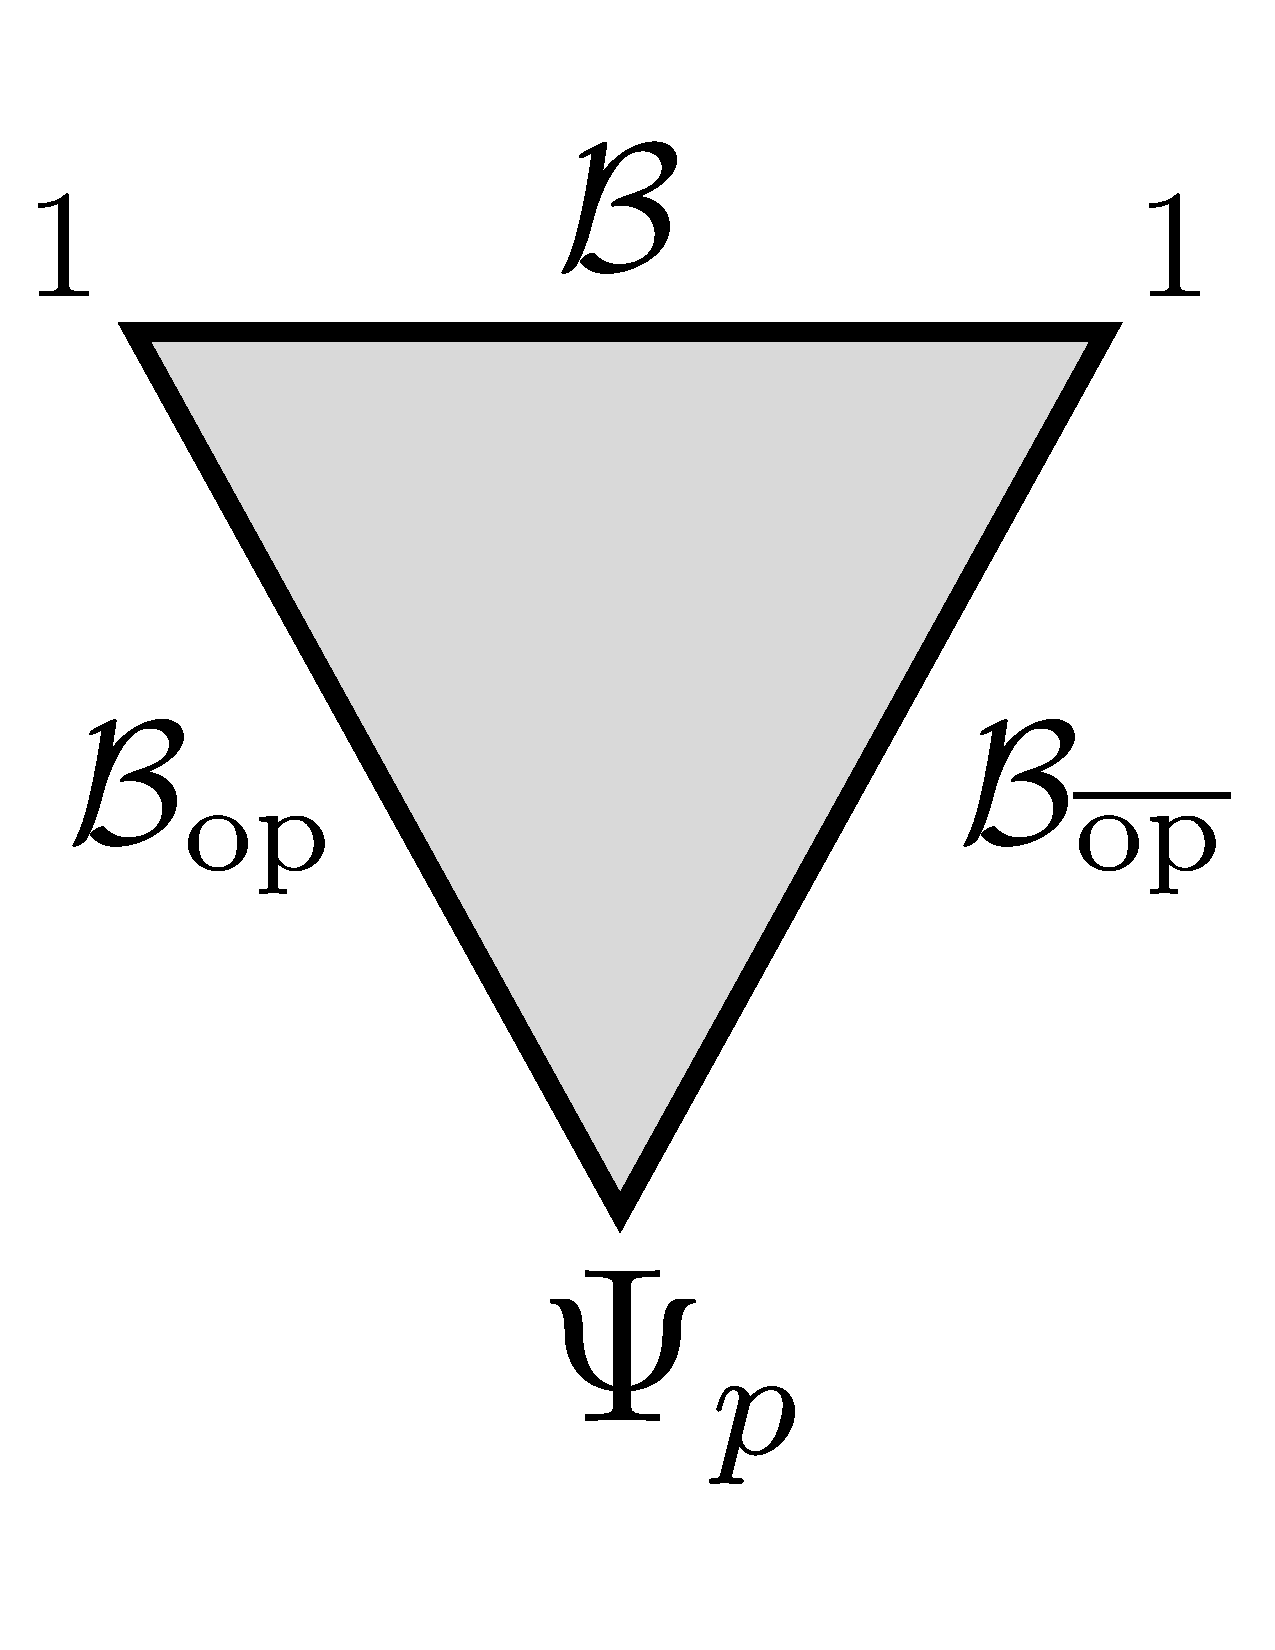
\includegraphics[width=1.2in]{Example10.pdf}
\end{center}
\caption{\small  一个三角形，其底角标以 $\Psi_p\in \Hom(\B_\bop,\B_\op)$，其余各角标以膜 $\B_\op$、$\B_\bop$ 与正则 Nahm 极点的对偶 $\B$ 之间的典范角。这个三角形上的路径积分计算 $(\chi,\Psi_p)$。 \label{example10}}
\end{figure}

我们加在 $\Psi_p$ 上的归一化条件还有另一种解释。我们在第 \ref{nbc} 节已说明，把 $\Psi_p$ 与 $A$-模型中由与正则 Nahm 极点（Nahm pole）相联系的膜 $\B_N$（带适当的角）所生成的态作内积是有意义的，尽管该膜的支撑完全在 $T^*\M(G,C)$ 之外。这个计算在 $B$-模型中其实相当直接。$\B_N$ 的 $B$-模型对偶就是 $\M_H$ 的结构层（structure sheaf）；也就是说，它是支撑为整个 $\M_H$、带平凡 $\CP$（Chan–Paton）丛的秩 1 膜 $\B$。$\B$ 与 $\B_\cc$ 有一个典范角，对应于两膜支撑之交（即 $\M_H\cap L_\op=L_\op$）上的常值函数 1。同样，$\B$ 与 $\bar\B_\cc$ 有一个典范角，由 $\M_H\cap L_{\bop}=L_{\bop}$ 上的函数 1 代表。设 $\chi\in \Hom(\bar\B_\cc,\B_\cc)$ 是由带这些典范角的膜 $\B$ 所生成的态。$B$-模型配对 $(\chi,\Psi_p)$ 由三角形（图 \ref{example10}）上的路径积分计算，该三角形的边标以膜 $\B$、$\B_\cc$ 与 $\bar\B_{\cc}$，其角标以 $\B$ 的典范角与态 $\Psi_p$。$B$-模型局域化到常值映射上；在此情形下，唯一满足必要条件的常值映射是把三角形映到点 $p$ 的常值映射。我们已取所有波函数都等于 1。因此 $(\chi,\Psi_p)=1$。换言之，Hitchin 哈密顿量的本征态 $\Psi_p$ 上那个导致此前关于其希尔伯特空间范数的预言的归一化条件，就是 $(\chi,\Psi_p)=1$。若能在 $A$-模型一侧计算 $(\chi,\Psi_p)$，就会纯粹以 $A$-模型的术语给出 $\Psi_p$ 希尔伯特空间范数的一个预言。配对 $(\chi,\Psi_p)$ 与几何朗兰兹的范畴化方法中的 Whittaker 系数（Whittaker coefficient）有些类似。
